\documentclass[platex,dvipdfmx]{jsarticle}
\usepackage{color}
\usepackage{listings,jvlisting}
\usepackage{graphicx}
\lstset{
  language=Python,
  basicstyle={\ttfamily},
  identifierstyle={\small},
  commentstyle={\small\itshape},
  keywordstyle={\small\bfseries\color{red}},
  ndkeywordstyle={\small},
  stringstyle={\small\ttfamily\color{yellow}},
  frame={tb},
  breaklines=true,
  columns=[l]{fullflexible},
  numbers=left,
  xrightmargin=0zw,
  xleftmargin=3zw,
  numberstyle={\scriptsize},
  stepnumber=1,
  numbersep=1zw,
  lineskip=-0.5ex
}
\renewcommand{\lstlistingname}{ソースコード}
\begin{document}
  \title{課題3レポート}
  \author{羽路 悠斗}
  \maketitle

  \section{課題内容}

  \subsection{誤差逆伝播法による3層ニューラルネットワークの学習}

  課題2のコードをベースに、3層ニューラルネットワークのパラメータ$W^{(1)}$ , $W^{(2)}$ , $b^{(1)}$ , $b^{(2)}$ を学習するプログラムを作成せよ。

  \begin{itemize}
    \item ネットワークの構造、バッチサイズは課題2と同じで良い
    \item 学習にはMNISTの学習データ60000枚を用いること
    \item 繰り返し回数は自由に決めて良い
    \item 学習率は自由に決めて良い
    \item 各エポックごとにクロスエントロピー誤差を標準出力に出力すること
    \item 学習終了時にパラメータをファイルに保存する機能を用意すること
    \item ファイルに保存したパラメータを読み込み、再利用できる機能を用意すること
  \end{itemize}

  \newpage

  \section{作成したプログラムの説明}
  
  \subsection{誤差逆伝播法}

  \subsubsection{設計方針}

  課題1、2にて各層の順伝播を関数として実装済みである。それらの戻り値を保持しておき、逆伝播を計算する。行(axis=0)がノードを表し、列(axis=1)がバッチサイズを表す入出力インターフェースであることに注意しておく。以下に、逆伝播の順序に従い、出力側から順に実装を示す。なお、これらは全てModelクラス中のtrain\_batch関数内に実装される。

  \subsubsection{ソフトマックス関数}

  ソフトマックス関数の順伝播である

  \begin{lstlisting}[caption=ex3.py, label=soft_fwd]
    y2 = self.softmax(a)
  \end{lstlisting}

  逆伝播である

  \begin{lstlisting}[caption=ex3.py, label=soft_bwd]
    diff_e_n_with_a = (y2 - tr_y.T)/self.batch_size # クラス数*bs
  \end{lstlisting}

  \subsubsection{全結合層2}

  二つ目の全結合層の順伝播である

  \begin{lstlisting}[caption=ex3.py, label=dense2_fwd]
    a = self.dense_layer2(y)
  \end{lstlisting}

  逆伝播である

  \begin{lstlisting}[caption=ex3.py, label=dense2_bwd]
    diff_e_n_with_y = self.w2.T @ diff_e_n_with_a # units*bs
    diff_e_n_with_w2 = diff_e_n_with_a @ y.T # クラス数*units
    diff_e_n_with_b2 = np.sum(diff_e_n_with_a, axis=1) # クラス数次元ベクトル
  \end{lstlisting}

  \subsubsection{シグモイド関数}

  シグモイド関数の順伝播である

  \begin{lstlisting}[caption=ex3.py, label=sig_fwd]
    y = self.sigmoid(t)
  \end{lstlisting}
  
  逆伝播である

  \begin{lstlisting}[caption=ex3.py, label=sig_bwd]
    diff_e_n_with_t = diff_e_n_with_y*(1-y)*y # units*bs
  \end{lstlisting}

  \subsubsection{全結合層1}

  一つ目の全結合層の順伝播である

  \begin{lstlisting}[caption=ex3.py, label=dense1_fwd]
    t = self.dense_layer1(x)
  \end{lstlisting}

  逆伝播である

  \begin{lstlisting}[caption=ex3.py, label=dense1_bwd]
    diff_e_n_with_x = self.w1.T @ diff_e_n_with_t # 784*bs
    diff_e_n_with_w1 = diff_e_n_with_t @ x.T # units*784
    diff_e_n_with_b1 = np.sum(diff_e_n_with_t, axis=1) # units数次元ベクトル
  \end{lstlisting}

  \subsubsection{重みの更新}

  パラメータは学習率と、パラメータの微分に基づいて更新される。

  \begin{lstlisting}[caption=ex3.py, label=update]
    self.w1 = self.w1 - lr*diff_e_n_with_w1
    self.b1 = self.b1 - lr*diff_e_n_with_b1
    self.w2 = self.w2 - lr*diff_e_n_with_w2
    self.b2 = self.b2 - lr*diff_e_n_with_b2
  \end{lstlisting}

  \subsubsection{バッチの学習}

  以上の処理をまとめたものがtrain\_batch関数である。

  \begin{lstlisting}[caption=ex3.py, label=train_batch]
    def train_batch(self, tr_x, tr_y, lr):
      x = self.input_layer(tr_x)
      t = self.dense_layer1(x)
      y = self.sigmoid(t)
      a = self.dense_layer2(y)
      y2 = self.softmax(a)
      e_n = self.cross_entropy(tr_y.T, y2)

      # 以下微分の形を行*列で示す
      diff_e_n_with_a = (y2 - tr_y.T)/self.batch_size # クラス数*bs
      diff_e_n_with_y = self.w2.T @ diff_e_n_with_a # units*bs
      diff_e_n_with_w2 = diff_e_n_with_a @ y.T # クラス数*units
      diff_e_n_with_b2 = np.sum(diff_e_n_with_a, axis=1) # クラス数次元ベクトル
      diff_e_n_with_t = diff_e_n_with_y*(1-y)*y # units*bs
      diff_e_n_with_x = self.w1.T @ diff_e_n_with_t # 784*bs
      diff_e_n_with_w1 = diff_e_n_with_t @ x.T # units*784
      diff_e_n_with_b1 = np.sum(diff_e_n_with_t, axis=1) # units数次元ベクトル

      # 重みの更新
      self.w1 = self.w1 - lr*diff_e_n_with_w1
      self.b1 = self.b1 - lr*diff_e_n_with_b1
      self.w2 = self.w2 - lr*diff_e_n_with_w2
      self.b2 = self.b2 - lr*diff_e_n_with_b2

      return e_n
  \end{lstlisting}

  \newpage

  \subsection{モデルの初期化と学習ループ}

  \subsubsection{初期化}
  モデルの初期化の際に、各層の重みを初期化する。

  \begin{lstlisting}[caption=ex3.py, label=init]
    class Model:
      def __init__(self) -> None:
        # モデルのアーキテクチャを作成
        self.units = 32
        self.batch_size = 100
        self.w1, self.b1 = random.normal(loc=0, scale=np.sqrt(1/784), size=784*self.units).reshape(self.units, 784), random.normal(loc=0, scale=np.sqrt(1/784), size=self.units)
        self.w2, self.b2 = random.normal(loc=0, scale=np.sqrt(1/self.units), size=self.units*10).reshape(10, self.units), random.normal(loc=0, scale=np.sqrt(1/self.units), size=10)
  \end{lstlisting}
  
  \subsubsection{学習ループ}

  学習ループは、学習データ、エポック数、学習率を受け取る関数として実装する。またエポック終了時に、そのエポックのミニバッチのクロスエントロピー誤差の平均を標準出力に出力する。デフォルト値として、エポック数10、学習率0.01を用いる。
  
  \begin{lstlisting}[caption=ex3.py, label=train]
      def train(self, train_x, train_y, epochs: int = 10, lr: float = 0.01):
        '''
        train_x: 学習データの特徴量
        train_y: 学習データのラベル
        epochs: エポック数
        lr: 学習率
        '''
        for i in tqdm(range(epochs)):
          entropies = []
          for j in range(60000//self.batch_size):
            tr_x, tr_y = self.preprocessing(train_x, train_y)
            entropies.append(self.train_batch(tr_x, tr_y, lr))
          print(f'Epoch {i+1} end! Cross entroppy is {sum(entropies)/len(entropies)}.')
  \end{lstlisting}

  \newpage

  \subsection{重みの保存と読み込み}

  \subsubsection{重みの保存}

  modelディレクトリを作成し、重みを保存する。

  \begin{lstlisting}[caption=ex3.py, label=save_model]
    def save_model(self, name):
      np.savez(f'model/{name}', w1=self.w1, b1=self.b1, w2=self.w2, b2=self.b2)
  \end{lstlisting}

  \subsubsection{重みの読み込み}

  modelディレクトリから、重みを読み込む。各パラメータについて、保存時の名前を明示する。

  \begin{lstlisting}[caption=ex3.py, label=load_model]
    def load_model(self, name):
      model = np.load(f'model/{name}.npz')
      self.w1, self.b1, self.w2, self.b2 = model['w1'], model['b1'], model['w2'], model['b2']
  \end{lstlisting}

  \newpage

  \section{実行結果}

  \begin{quote}
    実行部分は課題2と同様である

    \begin{lstlisting}[caption=ex3.py, label=main]
      if __name__ == '__main__': 
        train_x = mnist.download_and_parse_mnist_file('train-images-idx3-ubyte.gz')
        train_y = mnist.download_and_parse_mnist_file("train-labels-idx1-ubyte.gz")
        model = Model()
        model.train(train_x, train_y)
    \end{lstlisting}
  \end{quote}
  
  実行結果

  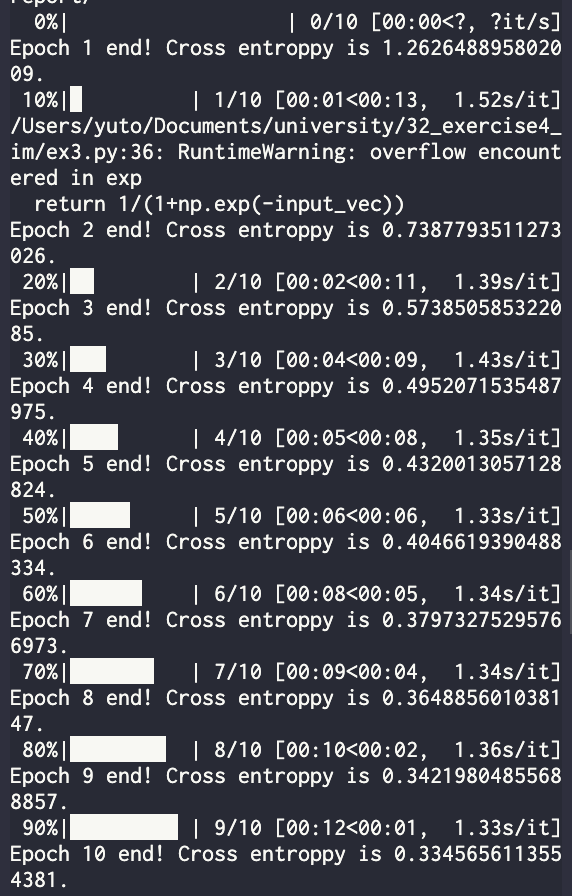
\includegraphics[]{ex3_output.png}

  クロスエントロピー誤差が減少していっている様子が観察できる。まだ収束しているとは言い難いのでエポック数を増やせばさらに損失を減らせると考えられる。

  \section{工夫点}

  各層の入力と出力のインターフェースを統一していたことで、逆伝播の実装も、テキストにあった式を愚直にnumpyで表現していくだけで済んだ。今回は学習ループが必要となったので、Modelクラスを作成し、外部からmodel.trainを呼ぶだけで良いようにした。このように、できる限り処理を切り分けるようにした。また今回も課題1、2と同様に、各層の演算にfor文を使わずに行列演算を駆使したことで、高速化できた。
  
  \section{問題点}

  逆伝播を関数化していないことや、層のパラメータをModelクラスが持っていることが、層の拡張性や、モデル構造の可変性を下げている。この問題は発展課題に取り組むにつれて顕在化した問題である。後の実装では、大幅に実装方針を変えて、これらの問題に対処した。
  
\end{document}